\begin{figure*}[t]
    \centering
    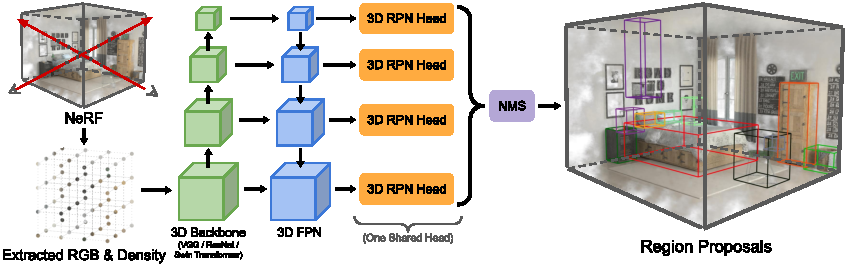
\includegraphics[width=0.95\linewidth]{figs/main_figure_2.pdf}
    \vspace{-0.1in}
    \caption{\textbf{NeRF-RPN.} Our \nerfrpn first samples a grid of points and extract their RGB and density in NeRF. The extracted volumetric features are then passed through a 3D backbone architecture to extract deep 3D features at multi-scale. The deep 3D features are fused using a 3D FPN module with a 3D RPN head to regress the potential region proposals.}\vspace{-0.2in}
    \label{fig:main}
    % \vspace{-0.1in}
    % redo: emphasize 3d convolution
    % anchor-free/based: another figure
\end{figure*}
